% -----------------------------------------------------------------------------
% Scattering foundations in strict SI units
% -----------------------------------------------------------------------------

场论计算首先给出约化振幅 $\mathcal M$，而实验记录的是事件率和截面。两者之间的桥梁完全由运动学与归一化决定：连续末态贡献质量壳相空间，总平移不变性给出四动量守恒的 $\delta$ 分布，最后除以入射通量才得到截面。因此一旦这套 SI 制相空间公式固定，QED、QCD 与 Standard Model 的区别只体现在代入的 $\mathcal M$。以下四动量始终采用全书统一的 SI 物理四动量
\begin{equation}
 p^\mu=\left(\frac{E_{\mathbf p}}{c},\mathbf p\right),
 \qquad
 p^2=m^2c^2,
 \qquad
 [p^\mu]=\mathrm{kg\,m\,s^{-1}}.
 \label{eq:si-scattering-fourmomentum-r9}
\end{equation}
因此 Mandelstam 变量具有动量平方量纲；截面中的面积量纲由显式的 \(\hbar^2\) 提供。四维积分限制到正能质量壳以后使用的基本测度是
\begin{equation}
 \boxed{
 \dd^4 p\,\delta(p^2-m^2c^2)\,\theta(p^0)
 =\frac{c\,\dd^3 p}{2E_{\mathbf p}}.}
 \label{eq:positive-energy-mass-shell-measure-r68}
\end{equation}
它说明连续末态的“态数”并不是普通的 \(\dd^3 p\)；因子 \(1/(2E_{\mathbf p})\) 正是 Lorentz 协变计数所要求的质量壳 Jacobian。

连续态统一采用 Wigner 单粒子表示的协变态归一化与完备关系 \eqnrefs{eq:rel-state-normalization-si-r9,eq:rel-completeness-si-r9}。Feynman 图经 LSZ 截肢后得到的约化不变量振幅记为 \(\mathcal M\)：外线 Dirac 旋量满足 \(\bar uu=2mc\)，而 \(2\to2\) 过程的 \(\mathcal M\) 取为无量纲。这个约定一旦与外腿留数一起固定，\(\hbar\) 与 \(c\) 的因子就不能再在振幅和截面之间任意移动。

对
\begin{equation*}
 p_1+p_2\longrightarrow p_3+p_4
\end{equation*}
定义
\begin{equation}
 \boxed{
 s=(p_1+p_2)^2,
 \qquad
 t=(p_1-p_3)^2,
 \qquad
 u=(p_1-p_4)^2.}
 \label{eq:mandelstam-def-si-r9}
\end{equation}
把三个定义相加并先只用四动量守恒 $p_1+p_2=p_3+p_4$，有
\begin{align*}
s+t+u
&=(p_1+p_2)^2+(p_1-p_3)^2+(p_1-p_4)^2\\
&=p_1^2+p_2^2+p_3^2+p_4^2,
\end{align*}
其中交叉项用 $p_2-p_3-p_4=-p_1$ 合并。再对四条外腿使用 $p_i^2=m_i^2c^2$，得到
\begin{equation}
 \boxed{
 s+t+u=(m_1^2+m_2^2+m_3^2+m_4^2)c^2.}
 \label{eq:stu-sum-si-r9}
\end{equation}
因此三个 Mandelstam 变量中只有两个独立；这是纯运动学约束，不依赖相互作用类型。
且质心总能量为
\begin{equation}
 E_{\rm cm}=c\sqrt{s}.
 \label{eq:Ecm-s-si-r9}
\end{equation}
因此 \(c\sqrt s\) 而非 \(\sqrt s\) 才具有能量量纲。


两体质心动量由 Källén 函数
\begin{equation*}
 \Lambda_K(a,b,c)\equiv a^2+b^2+c^2-2ab-2ac-2bc
\end{equation*}
统一给出：
\begin{equation}
 \boxed{
 |\mathbf p_i|
 =\frac{\sqrt{\Lambda_K(s,m_1^2c^2,m_2^2c^2)}}{2\sqrt s},
 \qquad
 |\mathbf p_f|
 =\frac{\sqrt{\Lambda_K(s,m_3^2c^2,m_4^2c^2)}}{2\sqrt s}.}
 \label{eq:cm-momenta-kallen-si-r9}
\end{equation}
根号非负同时给出末态阈值 \(c\sqrt s\ge(m_3+m_4)c^2\)。

为避免在四维 \(\delta\) 函数中混合动量与能量单位，定义能量四矢量
\begin{equation*}
 \mathcal P^\mu\equiv cp^\mu=(E,c\mathbf p).
\end{equation*}
二体 Lorentz 不变相空间于是定义为
\begin{equation}
 \dd\mathfrak P_2
 =(2\pi)^4\delta^{(4)}(\mathcal P_1+\mathcal P_2-\mathcal P_3-\mathcal P_4)
 \prod_{a=3,4}\frac{c^3\dd^3 p_a}{(2\pi)^3\,2E_a},
 \label{eq:phase2-si-start-r9}
\end{equation}
在质心系化为
\begin{equation}
 \boxed{
 \dd\mathfrak P_2
 =\frac1{16\pi^2}\frac{|\mathbf p_f|}{\sqrt s}\,\dd\Omega.}
 \label{eq:phase2-final-si-r9}
\end{equation}
这里 \(|\mathbf p_f|/\sqrt s\) 无量纲。

截面还需要一个“单位入射束流”的定义。非相对论情况下常用两束粒子的相对速度，但普通三速度差不是 Lorentz 标量。由两条入射四动量可以构造
\begin{equation}
 \mathcal I_{12}
 \equiv\sqrt{(p_1\!\cdot p_2)^2-m_1^2m_2^2c^4}
 \label{eq:invariant-flux-scalar-r9}
\end{equation}
它在任意惯性系给出同一个入射通量因子。把它换算成速度量纲后定义
\begin{equation}
 v_{\rm M}
 \equiv
 \frac{c^3\mathcal I_{12}}{E_1E_2}.
 \label{eq:moller-velocity-si-r9}
\end{equation}
这个量传统上称为 M\o ller 相对速度；名称本身并不增加新的物理假设。它在质心系满足 \(\mathcal I_{12}=|\mathbf p_i|\sqrt s\)，并恰好退化成两条轨迹的相对相遇速度。

连续态的平方 \(\delta\) 函数必须由有限空间盒和有限观测时间定义。若初态与末态的总能量分别为 $E_i$ 与 $E_f$，先定义能量失配
\begin{equation*}
 \delta E\equiv E_f-E_i,\qquad [\delta E]=\mathrm J.
\end{equation*}
能量守恒就是 $\delta E=0$。取体积 \(V\) 与观测时间 \(T\)，则
\begin{equation}
 (2\pi\hbar)^3\delta^{(3)}(\mathbf0)=V,
 \qquad
 \sum_{\mathbf p}\longrightarrow
 V\int\frac{\dd^3 p}{(2\pi\hbar)^3},
 \label{eq:box-delta-density-r15}
\end{equation}
以及
\begin{equation}
 \lim_{T\to\infty}\frac1T
 \left|\int_{-T/2}^{T/2}\dd t\,\ee^{\ii\delta E t/\hbar}\right|^2
 =2\pi\hbar\delta(\delta E).
 \label{eq:delta-square-time-r15}
\end{equation}
有限时空调节先把 $S$ 矩阵元的平方变成“单位时间、单位盒中一对入射粒子”的跃迁率；这还不是截面，因为其中仍含任意盒体积。只有再除以同一归一化下的入射通量密度，$V$ 才会消失并留下可与实验比较的面积。由此先得到二体末态跃迁率
\begin{equation}
 \boxed{
 \dd\Gamma_{1+2\to2}
 =\frac{\hbar^2c^3}{4VE_1E_2}
 \overline{|\mathcal M|^2}\,\dd\mathfrak P_2.}
 \label{eq:box-transition-rate-r15}
\end{equation}
除以入射通量密度 \(v_{\rm M}/V\)，便得到后续所有 \(2\to2\) 过程共用的截面母式
\begin{equation}
 \boxed{
 \frac{\dd\sigma}{\dd\Omega}
 =\frac{\hbar^2}{64\pi^2s}
 \frac{|\mathbf p_f|}{|\mathbf p_i|}
 \overline{|\mathcal M|^2}.}
 \label{eq:2to2-cross-section-master-si-r9}
\end{equation}
固定 \(s\) 时，\(t=(p_1-p_3)^2\) 对散射角的依赖完全由二体运动学决定。把角变量换成 \(t\)，同一截面母式可以写成
\begin{equation}
 \boxed{
 \frac{\dd\sigma}{\dd t}
 =\frac{\hbar^2\overline{|\mathcal M|^2}}
 {16\pi\Lambda_K(s,m_1^2c^2,m_2^2c^2)}.}
 \label{eq:2to2-dsigma-dt-si-r68}
\end{equation}
这个形式在比较不同交换道或直接以 Mandelstam 变量积分时更方便；它没有引入新的动力学假设，只是把\eqnrefs{eq:2to2-cross-section-master-si-r9} 的角变量重新参数化。末态若含 \(N\) 个完全相同、而相空间又以有序标签积分的粒子，还需除以 \(N!\) 消除重复计数。

对等质量弹性散射 \(m_1=m_2=m_3=m_4=m\)，在质心系取
\begin{equation*}
p_1=(E/c,\mathbf p),\quad p_2=(E/c,-\mathbf p),\quad
p_3=(E/c,\mathbf p'),\quad p_4=(E/c,-\mathbf p'),
\end{equation*}
其中 $|\mathbf p'|=|\mathbf p|\equiv p$、$\mathbf p\cdot\mathbf p'=p^2\cos\theta$。于是
\begin{equation*}
(p_1-p_3)^2=-|\mathbf p-\mathbf p'|^2,
\qquad
(p_1-p_4)^2=-|\mathbf p+\mathbf p'|^2,
\end{equation*}
再用 $E^2=m^2c^4+p^2c^2$ 代入并整理，得到
\begin{equation}
 \boxed{
 t=-2p^2(1-\cos\theta),
 \qquad
 u=-2p^2(1+\cos\theta),
 \qquad
 s=4(m^2c^2+p^2).}
 \label{eq:t-u-cm-equalmass-si-r9}
\end{equation}
具体相互作用只通过 \(\mathcal M(s,t,u)\) 进入，不改变这些运动学关系。

同一有限时间归一化给出质量为 \(M\) 的一体初态衰变母式
\begin{equation}
 \boxed{
 \dd\Gamma_{1\to n}
 =\frac{1}{2M\hbar}
 \overline{|\mathcal M|^2}\,\dd\mathfrak P_n.}
 \label{eq:master-decay-rate-si-r9}
\end{equation}
散射截面与衰变率因此共享同一套连续态归一化、质量壳测度和 LSZ 振幅约定，而不是两套互不相干的记忆公式。


三体末态第一次引入一个两体末态没有的新自由度：即使总四动量已经固定，三个末态粒子之间仍可连续重新分配内部不变质量。为把这个自由度显式化，定义
\begin{equation}
 \mathcal S_{ij}
 \equiv \bigl[c(p_i+p_j)\bigr]^2
 =c^2(p_i+p_j)^2,
 \qquad [\mathcal S_{ij}]=\mathrm{J^2}.
 \label{eq:threebody-invariant-mass-energy2-dp52}
\end{equation}
设质量为 $M$ 的母粒子衰变为 $1+2+3$，并令
$q_{12}\equiv p_1+p_2$、$\mathcal Q_{12}\equiv c q_{12}$。三体 Lorentz 不变相空间本身仍由三条单粒子质量壳测度和一个总四动量 $\delta$ 函数组成：
\begin{equation}
 \boxed{
 \dd\mathfrak P_3
 =(2\pi)^4\delta^{(4)}
 (\mathcal P-\mathcal P_1-\mathcal P_2-\mathcal P_3)
 \prod_{i=1}^{3}
 \frac{\dd^3 \boldsymbol{\mathcal P}_i}{(2\pi)^3 2E_i}.}
 \label{eq:phase3-definition-dp68}
\end{equation}
要把内部不变质量 $\mathcal S_{12}$ 显式取作积分变量，只需在\eqnrefs{eq:phase3-definition-dp68} 中插入恒等分解
\begin{equation*}
 1=\int\frac{\dd\mathcal S_{12}}{2\pi}
 \int\frac{\dd^4 \mathcal Q_{12}}{(2\pi)^4}
 (2\pi)^4\delta^{(4)}(\mathcal Q_{12}-c p_1-c p_2)
 (2\pi)\delta(\mathcal Q_{12}^2-\mathcal S_{12})\theta(\mathcal Q_{12}^0),
\end{equation*}
便可把三体问题递归拆成两个二体问题：
\begin{equation}
 \boxed{
 \dd\mathfrak P_3(P;1,2,3)
 =\frac{\dd\mathcal S_{12}}{2\pi}\,
 \dd\mathfrak P_2(P;q_{12},3)\,
 \dd\mathfrak P_2(q_{12};1,2).}
 \label{eq:phase3-recursive-dp52}
\end{equation}
这个分解的物理含义很直接：先把母粒子看成衰变为“质量为 $\sqrt{\mathcal S_{12}}/c^2$ 的复合中间系统 $q_{12}$”和粒子 3，再在 $q_{12}$ 的静止系中让它衰变为粒子 1 与 2。$q_{12}=p_1+p_2$ 是对同一三体运动学作 $(12)+3$ 分组时引入的复合四动量坐标。

若母粒子无自旋，或已对其自旋取平均，则整体空间方向没有物理信息。积分掉整体转动自由度后，可直接用两项独立的不变质量平方作为 Dalitz 坐标：
\begin{equation}
 \boxed{
 \dd\mathfrak P_3
 =\frac{\dd\mathcal S_{12}\,\dd\mathcal S_{23}}
 {128\pi^3 M^2c^4}.}
 \label{eq:phase3-dalitz-dp52}
\end{equation}
因此三体相空间的非平凡内容全部进入 Dalitz 区域的边界，而不是测度中的复杂权重；若实验 Dalitz 图内部出现非均匀事件密度，它来自振幅的动力学权重而不是这一 Jacobian。要得到边界，只需在 $q_{12}$ 的静止系中观察粒子 2 与粒子 3 的夹角 $\theta^*$。此时
\begin{equation}
 \boxed{
 \mathcal S_{23}
 =m_2^2c^4+m_3^2c^4
 +2\left(E_2^*E_3^*
 -c^2|\mathbf p_2^*||\mathbf p_3^*|\cos\theta^*\right).}
 \label{eq:dalitz-angular-map-dp68}
\end{equation}
星号只表示在 $q_{12}$ 静止系取值。物理角满足 $-1\le\cos\theta^*\le1$，因此固定 $\mathcal S_{12}$ 时，$\mathcal S_{23}$ 的上下界为
\begin{align}
 \mathcal S_{23}^{\pm}(\mathcal S_{12})
 ={}&m_2^2c^4+m_3^2c^4
 +\frac{1}{2\mathcal S_{12}}
 \Bigl[
 (\mathcal S_{12}+m_2^2c^4-m_1^2c^4)
 (M^2c^4-\mathcal S_{12}-m_3^2c^4)
 \nonumber\\
 &\qquad\qquad
 \pm
 \sqrt{\Lambda_K(\mathcal S_{12},m_1^2c^4,m_2^2c^4)}
 \sqrt{\Lambda_K(M^2c^4,\mathcal S_{12},m_3^2c^4)}
 \Bigr].
 \label{eq:dalitz-boundary-dp52}
\end{align}
这里同一个 K\"all\'en 函数同时控制“$1+2$ 子系统能否形成”以及“该子系统能否与粒子 3 共同来自母粒子”两个阈值。

\begin{exbox}[无质量三体末态的 Dalitz 三角形]
取 $m_1=m_2=m_3=0$。三项不变质量满足
\begin{equation*}
 \mathcal S_{12}+\mathcal S_{23}+\mathcal S_{13}=M^2c^4,
 \qquad
 \mathcal S_{ij}\ge0.
\end{equation*}
因此物理区域就是
\begin{equation*}
 \mathcal S_{12}\ge0,
 \qquad
 \mathcal S_{23}\ge0,
 \qquad
 \mathcal S_{12}+\mathcal S_{23}\le M^2c^4
\end{equation*}
围成的直角三角形。除去母粒子质量尺度后，定义无量纲坐标
\begin{equation*}
 x\equiv\frac{\mathcal S_{12}}{M^2c^4},
 \qquad
 y\equiv\frac{\mathcal S_{23}}{M^2c^4}.
\end{equation*}
于是三个顶点依次为 $(0,0)$、$(1,0)$、$(0,1)$，物理区域满足 $x\ge0$、$y\ge0$、$x+y\le1$，无量纲面积恰为 $1/2$：
\begin{equation*}
 \int_0^1\dd x\int_0^{1-x}\dd y=\frac12.
\end{equation*}
\begin{center}
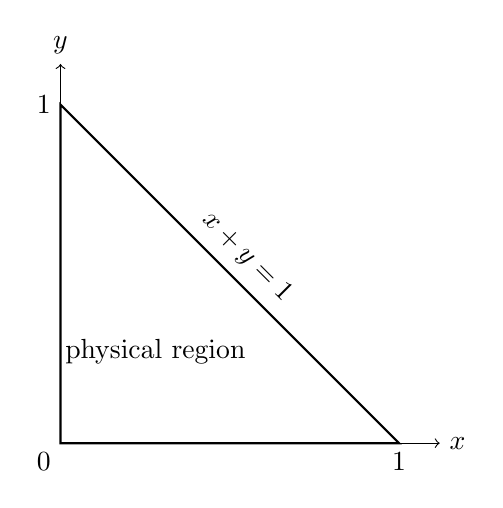
\begin{tikzpicture}[x=4.3cm,y=4.3cm]
  \draw[->] (0,0)--(1.12,0) node[right] {$x$};
  \draw[->] (0,0)--(0,1.12) node[above] {$y$};
  \draw[thick] (0,0)--(1,0)--(0,1)--cycle;
  \node[below left] at (0,0) {$0$};
  \node[below] at (1,0) {$1$};
  \node[left] at (0,1) {$1$};
  \node[rotate=-45,fill=white,inner sep=1pt] at (0.55,0.55) {$x+y=1$};
  \node at (0.28,0.27) {physical region};
\end{tikzpicture}
\end{center}
若截肢振幅在这个区域内近似为常数，三体相空间在 $(x,y)$ 平面上的事件密度就是常数，所以归一化后的二维密度为 $2$。任何明显的条带、边缘增强或局域峰都必须来自振幅本身的传播子、共振或角动量结构，而不是来自这个无质量三体测度的运动学边界。
\end{exbox}
